\pagestyle{fancy}
\fancyhead[l]{\autorUO}
\fancyfoot[l]{\asignaturaAbbr}
\fancyfoot[r]{\fecha}

\section{\pytorch} \label{sec:intro_pytorch}
\pytorch\footnote{\url{https://pytorch.org/}} es una biblioteca de cómputo científico diseñada principalmente para el desarrollo de algoritmos de
aprendizaje automático, aunque su estructura y diseño la convierten en una herramienta muy versátil para el cálculo numérico general y el procesamiento
de datos de alta dimensión.

\subsection{Instalación} \label{sec:intro_install}
Redactar...

\begin{lstlisting}[language=bash, caption={Comando de instalación de \pytorch\ con soporte CUDA 13.0}, label={lst: intro_install_pytorch}]
pip3 install torch torchvision --index-url https://download.pytorch.org/whl/cu130
\end{lstlisting}

\begin{lstlisting}[language=python, caption={Código de prueba de instalación de \pytorch}, label={lst: intro_test_pytorch}]
import torch
x = torch.rand(5, 3)
print(x)
print(torch.cuda.is_available())
\end{lstlisting}

\begin{lstlisting}[language=bash, caption={Salida esperada del código de prueba de instalación de \pytorch}, label={lst: intro_test_pytorch_output}]
tensor([[0.6557, 0.0198, 0.0169],
        [0.0468, 0.2888, 0.0026],
        [0.4243, 0.1107, 0.6735],
        [0.1006, 0.6152, 0.9174],
        [0.1755, 0.9582, 0.8951]])
True
\end{lstlisting}

\begin{lstlisting}[language=bash, caption={Comando de instalación de \textit{h5py}}, label={lst: intro_install_h5py}]
pip install h5py
\end{lstlisting}

\subsubsection{Instalación de \texttt{ipykernel}} \label{sec:intro_ipykernel}
\begin{lstlisting}[language=bash, caption={Instalación de \texttt{ipykernel} en un entorno virtual de \texttt{pyenv}} , label={lst:install_ipykernel}]
pip install ipykernel
\end{lstlisting}

\newpage
\subsection{Tensores} \label{sec:intro_tensors}
Los \textit{tensores} son la base fundamental de \pytorch. Se trata de entidades multidimensionales capaces de representar información numérica de
forma compacta y eficiente, permitiendo la ejecución de operaciones matemáticas optimizadas tanto en CPU como en GPU. Desde un punto
de vista matemático, un tensor puede entenderse como una generalización de los vectores y las matrices a espacios de dimensión superior.

Como se muestra en la \autoref{eq:tensor_formal}, un tensor de orden $n$ puede expresarse como:

\begin{myequation}
	\begin{equation}
		T_{i_1 i_2 \ldots i_n} \in \mathbb{R}^{d_1 \times d_2 \times \ldots \times d_n}
		\label{eq:tensor_formal}
	\end{equation}
	\myequations{Representación formal de un tensor de orden $n$.}
	\caption{Representación formal de un tensor de orden $n$}
\end{myequation}

donde cada índice $i_k$ recorre una dimensión $d_k$ del espacio de datos. Así, un escalar puede considerarse un tensor de orden 0,
un vector un tensor de orden 1 y una matriz un tensor de orden 2. Esta generalización permite extender las operaciones algebraicas
clásicas a dominios de mayor complejidad, conservando propiedades como la linealidad y la composicionalidad.

Los tensores en \pytorch\ no solo almacenan datos, sino que también encapsulan información sobre su tipo de dato
(\texttt{dtype}), dispositivo de ejecución (\texttt{device}) y forma (\texttt{shape}). Esta estructura interna los convierte en
objetos altamente versátiles para el procesamiento numérico y gráfico, especialmente en contextos donde el rendimiento computacional
es de vital importancia.

\subsection{Operaciones con tensores} \label{sec:intro_tensor_operations}
La biblioteca proporciona una amplia gama de transformaciones algebraicas y funcionales que pueden ejecutarse de manera vectorizada,
evitando la iteración explícita y aprovechando la paralelización inherente al hardware.

Las operaciones básicas incluyen la suma, resta, multiplicación escalar, producto punto y producto matricial. Además, \pytorch\
permite realizar operaciones más avanzadas como transposición, cambio de forma (\texttt{reshape}), concatenación y reducción,
todas optimizadas internamente para ejecutarse con la máxima eficiencia posible.

Desde el punto de vista algebraico, estas operaciones preservan las propiedades fundamentales de la linealidad, de modo que
para dos tensores $A$ y $B$ y un escalar $\alpha$ se cumple que, como se muestra en la \autoref{eq:tensor_linearity}:

\begin{myequation}
	\begin{equation}
		\alpha(A + B) = \alpha A + \alpha B
		\label{eq:tensor_linearity}
	\end{equation}
	\myequations{Propiedad de linealidad en operaciones con tensores.}
	\caption{Propiedad de linealidad en operaciones con tensores}
\end{myequation}

El modelo de ejecución de \pytorch\ está diseñado para que todas las operaciones sobre tensores sean consistentes en
términos de dimensiones y tipos, lo que facilita el diseño modular de algoritmos numéricos. Además, el motor interno de la
biblioteca realiza comprobaciones automáticas de compatibilidad entre dimensiones, lanzando excepciones cuando las operaciones
no son válidas.

\newpage
\subsection{Representación de imágenes con tensores} \label{sec:intro_image_tensors}
Una de las aplicaciones más relevantes de los tensores en el contexto de este Trabajo Fin de Máster es la representación de imágenes digitales.
En \pytorch, una imagen se modela como un tensor tridimensional $I \in \mathbb{R}^{C \times H \times W}$, donde $C$
representa el número de canales de color (por ejemplo, $C = 3$ para imágenes RGB), $H$ la altura y $W$ el ancho.

Cada elemento $I_{c,h,w}$ del tensor almacena la intensidad del píxel ubicado en la posición $(h, w)$ del canal $c$. Esta representación
facilita la manipulación matemática de imágenes, permitiendo aplicar transformaciones geométricas, filtrados y operaciones convolucionales
mediante simples operaciones tensoriales. Puede observarse una representación conceptual de una imagen RGB como tensor tridimensional en la
\autoref{fig:image_tensor}.

\begin{figure}[h]
	\centering
	% --- Subfigure 1 ---
	\begin{subfigure}[b]{0.45\textwidth}
		\centering
		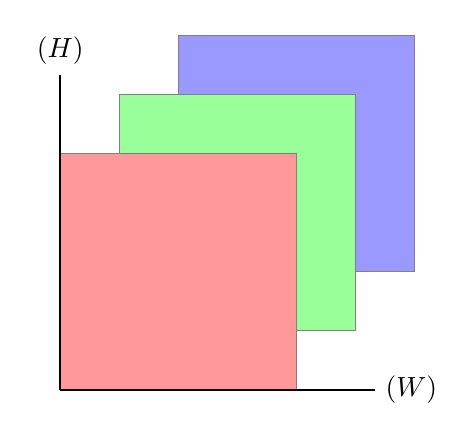
\begin{tikzpicture}
			[
				x={(1cm, 0cm)},
				y={(0cm, 1cm)},
				z={(0.5cm, 0.5cm)}
			]
			% RGB Planes
			\foreach \z/\color in {3/blue!40, 1.5/green!40, 0/red!40} {
					\filldraw[fill=\color, draw=black!50]
					(0,0,\z) -- ++(3,0,0) -- ++(0,3,0) -- ++(-3,0,0) -- cycle;
				}
			% Edges
			\draw[thick] (0,0,0) -- (4,0,0) node[right] {\textrm{($W$)}};
			\draw[thick] (0,0,0) -- (0,4,0) node[above] {\textrm{($H$)}};
		\end{tikzpicture}
		\caption{}
	\end{subfigure}
	\hfill
	% --- Subfigure 2 ---
	\begin{subfigure}[b]{0.45\textwidth}
		\centering
		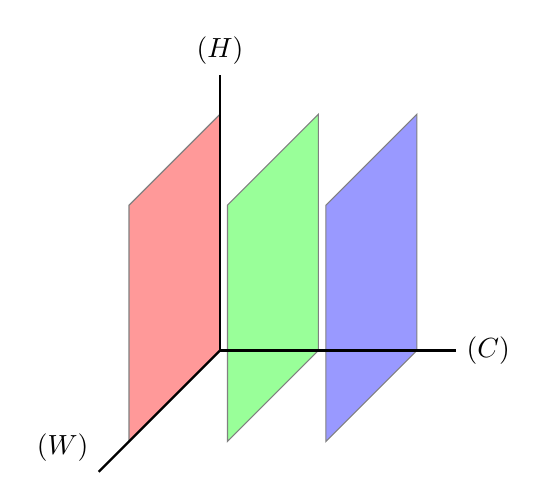
\begin{tikzpicture}
			% RGB Planes
			\foreach \z/\color in {0/red!40,1.25/green!40,2.5/blue!40} {
					\filldraw[fill=\color, draw=black!50]
					(\z,0,0) -- ++(0,3,0) -- ++(0,0,3) -- ++(0,-3,0) -- cycle;
				}
			% Edges
			\draw[thick] (0,0,0) -- (3,0,0) node[right] {\textrm{($C$)}};
			\draw[thick] (0,0,0) -- (0,3.5,0) node[above] {\textrm{($H$)}};
			\draw[thick] (0,0,0) -- (0,0,4) node[above left] {\textrm{($W$)}};
		\end{tikzpicture}
		\caption{}
	\end{subfigure}
	\caption{Representación conceptual de una imagen RGB como tensor tridimensional}
	\label{fig:image_tensor}
\end{figure}

Numéricamente, una imagen RGB de tamaño $3 \times 3$ píxeles puede representarse como el tensor $I$ de forma $[3, 3, 3]$, donde
cada canal de color contiene una matriz bidimensional con los valores de intensidad correspondientes.
En la \autoref{fig:image_tensor_example} se muestra un ejemplo concreto de esta representación.

\begin{figure}[h]
	\centering
	\begin{minipage}{0.6\textwidth}
		\[
			I =
			\left[
				\begin{array}{l}
					\text{R} =
					\begin{bmatrix}
						255 & 128 & 64 \\
						32  & 16  & 8  \\
						4   & 2   & 1
					\end{bmatrix},  \\[2em]
					\text{G} =
					\begin{bmatrix}
						0   & 64  & 128 \\
						192 & 255 & 128 \\
						64  & 32  & 16
					\end{bmatrix}, \\[2em]
					\text{B} =
					\begin{bmatrix}
						10 & 20 & 30 \\
						40 & 50 & 60 \\
						70 & 80 & 90
					\end{bmatrix}
				\end{array}
				\right]
		\]
	\end{minipage}
	\caption{Ejemplo de representación tensorial de una imagen RGB de $3 \times 3$ píxeles}
	\label{fig:image_tensor_example}
\end{figure}

\newpage
\subsubsection{Leyendo imágenes: \textit{imageio}} \label{sec:intro_imageio}
\textit{imageio}\footnote{\url{https://imageio.github.io/}} es una biblioteca de Python que facilita la lectura y escritura de 
imágenes en una amplia variedad de formatos.

[...]

\begin{lstlisting}[language=bash, caption={Comando de instalación de \textit{imageio}}, label={lst: intro_install_imageio}]
pip install imageio
\end{lstlisting}

\subsection{Tensores en GPU} \label{sec:intro_tensors_gpu}
[...]

